
% !TEX TS-program = pdflatex
% !TEX encoding = UTF-8 Unicode

% This is a simple template for a LaTeX document using the "article" class.
% See "book", "report", "letter" for other types of document.

\documentclass[11pt]{article} % use larger type; default would be 10pt

\usepackage[utf8]{inputenc} % set input encoding (not needed with XeLaTeX)

%%% Examples of Article customizations
% These packages are optional, depending whether you want the features they provide.
% See the LaTeX Companion or other references for full information.

%%% PAGE DIMENSIONS
\usepackage{geometry} % to change the page dimensions
\geometry{a4paper} % or letterpaper (US) or a5paper or....
% \geometry{margin=2in} % for example, change the margins to 2 inches all round
% \geometry{landscape} % set up the page for landscape
%   read geometry.pdf for detailed page layout information

\usepackage{graphicx} % support the \includegraphics command and options

% \usepackage[parfill]{parskip} % Activate to begin paragraphs with an empty line rather than an indent

%%% PACKAGES
\usepackage{booktabs} % for much better looking tables
\usepackage{array} % for better arrays (eg matrices) in maths
\usepackage{paralist} % very flexible & customisable lists (eg. enumerate/itemize, etc.)
\usepackage{verbatim} % adds environment for commenting out blocks of text & for better verbatim
\usepackage{subfig} % make it possible to include more than one captioned figure/table in a single float
% These packages are all incorporated in the memoir class to one degree or another...

%%% HEADERS & FOOTERS
\usepackage{fancyhdr} % This should be set AFTER setting up the page geometry
\pagestyle{fancy} % options: empty , plain , fancy
\renewcommand{\headrulewidth}{0pt} % customise the layout...
\lhead{}\chead{}\rhead{}
\lfoot{}\cfoot{\thepage}\rfoot{}

%%% SECTION TITLE APPEARANCE
\usepackage{sectsty}
\allsectionsfont{\sffamily\mdseries\upshape} % (See the fntguide.pdf for font help)
% (This matches ConTeXt defaults)

%%% ToC (table of contents) APPEARANCE
\usepackage[nottoc,notlof,notlot]{tocbibind} % Put the bibliography in the ToC
\usepackage[titles,subfigure]{tocloft} % Alter the style of the Table of Contents
\renewcommand{\cftsecfont}{\rmfamily\mdseries\upshape}
\renewcommand{\cftsecpagefont}{\rmfamily\mdseries\upshape} % No bold!

%%% END Article customizations

%%% The "real" document content comes below...

\title{Brief Article}
\author{The Author}
%\date{} % Activate to display a given date or no date (if empty),
         % otherwise the current date is printed 

\begin{document}
%\maketitle



\begin{figure}[h!]
\begin{center}
  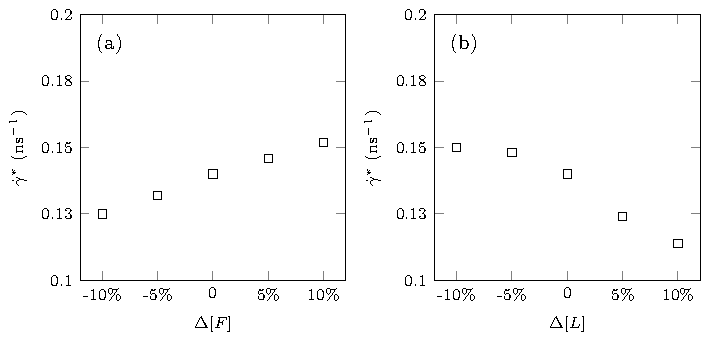
\includegraphics[height=0.3\textheight]{ChangeLengthForce.pdf}
\end{center}
\begin{caption}{\label{fig:PramChange}
  Panel (a) shows a linear relationship between change of force parameters and the critical shear rate $\dot\gamma^*$. 
  %
  Panel (b) provides numerical results of critical shear rates $\dot\gamma^*$ when the length parameters are adjusted.}
\end{caption}
\end{figure}


The rheology study has shown that the striated structure under shear and Taylor-Green flows exhibit a shear-thinning behavior.
To further quantify the contest between shear and head-tail attraction, we found that a 5\% and 10\% relative increases in the parameters $\gamma$ and
$M$ resulted in 4.29\% and 8.57\% relative increases in critial shear rate $\dot\gamma$, from 0.14 to 0.0.146 and 0.14 to 0.152, respectively. 
A proportional relationship is observed as the parameters decrease and it is shown in Figure~\ref{fig:PramChange}(a).
Moreover, Figure~\ref{fig:PramChange}(b) shows that 5\% and 10\% decreases in the particle radius c, screening length $\rho$ and repulsion distance $\rho_0$ gave 5.71\%  and 7.14\% increase in $\dot\gamma$ from 0.14 to 0.148 and 0.14 to 0.15.
In addition, 5\% and 10\% increases in length parameters gave 11.43\% and 18.57\% decrease in critical shear rate $\dot\gamma$.
The overall result provides another evidence that a different hydrophobicity suggests an unalike rheology and dynamics viscosity from the suspended vesicle experiments.


\end{document}
